\subsubsection{I}
We design a I controller with siso tool box.
$$
C(s) = \dfrac{1}{s}
$$
\begin{itemize}
	\item all figures from siso toolbox
	\begin{figure}[H]
		\caption{All figures from siso toolbox}
		\centering
		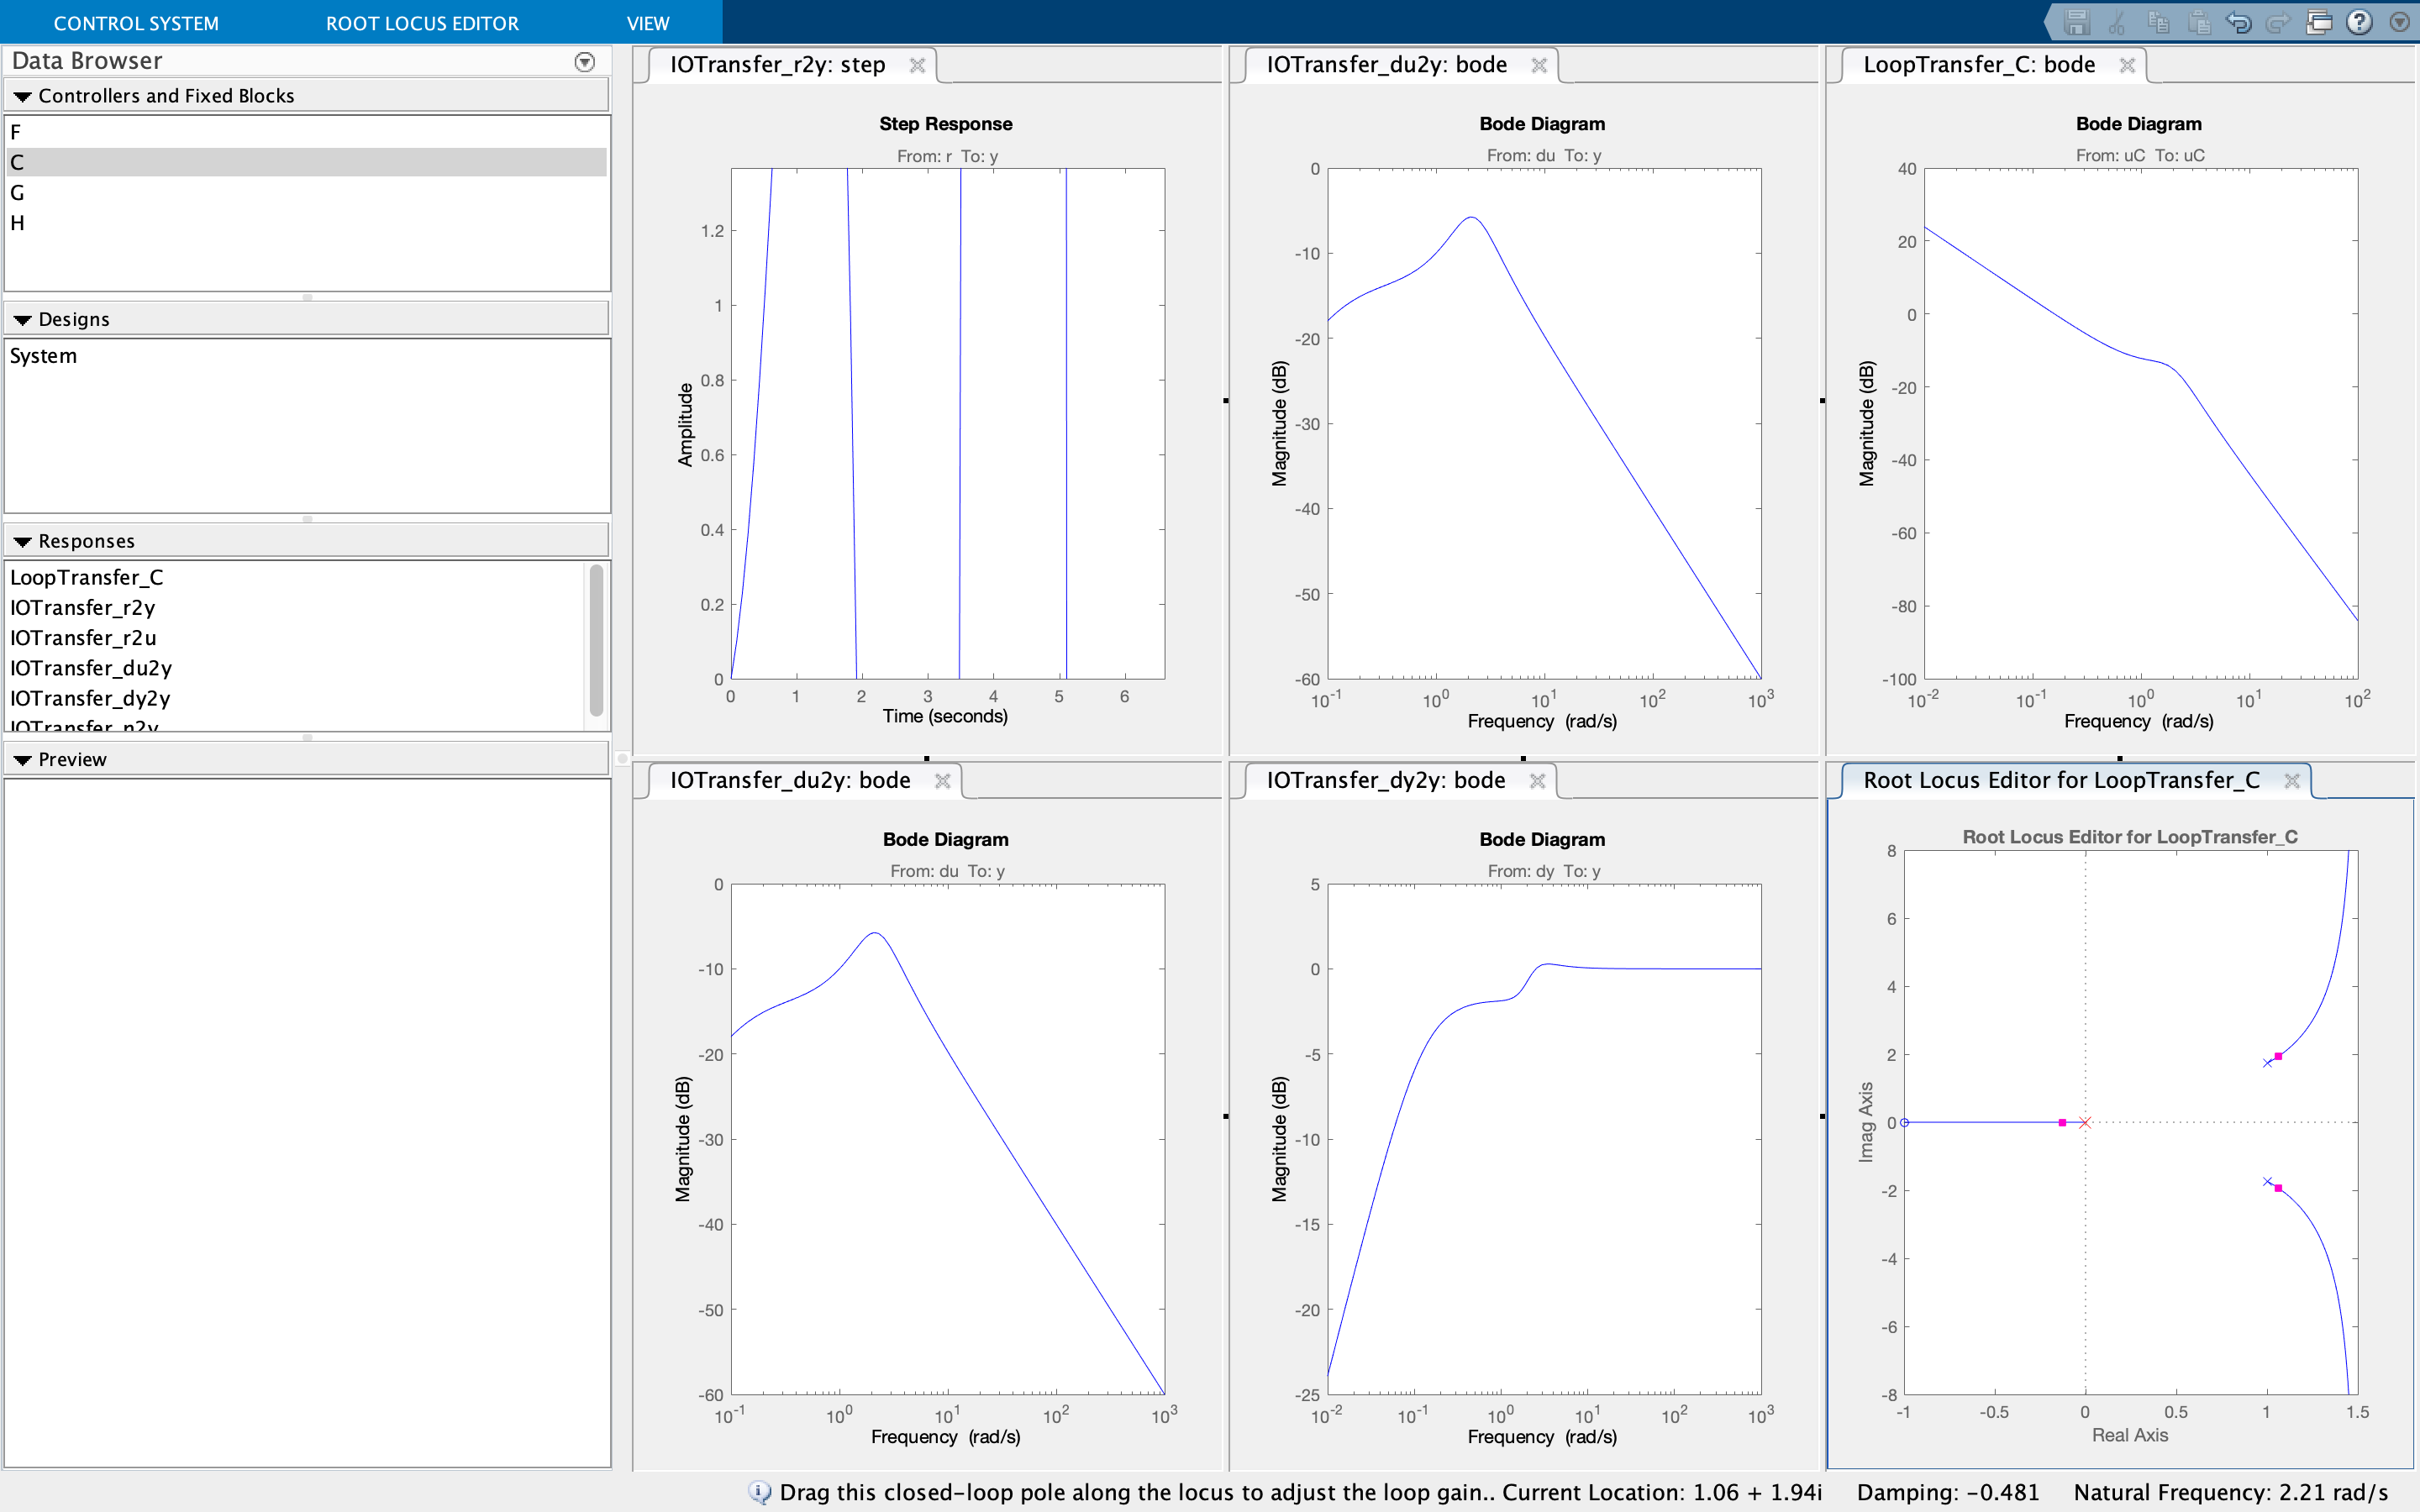
\includegraphics[width=16cm]{../Figure/Q1/Q1_b/I/siso_all.png}
	\end{figure}
	\newpage
	\item root locus with I controller
	\begin{figure}[H]
		\caption{root locus}
		\centering
		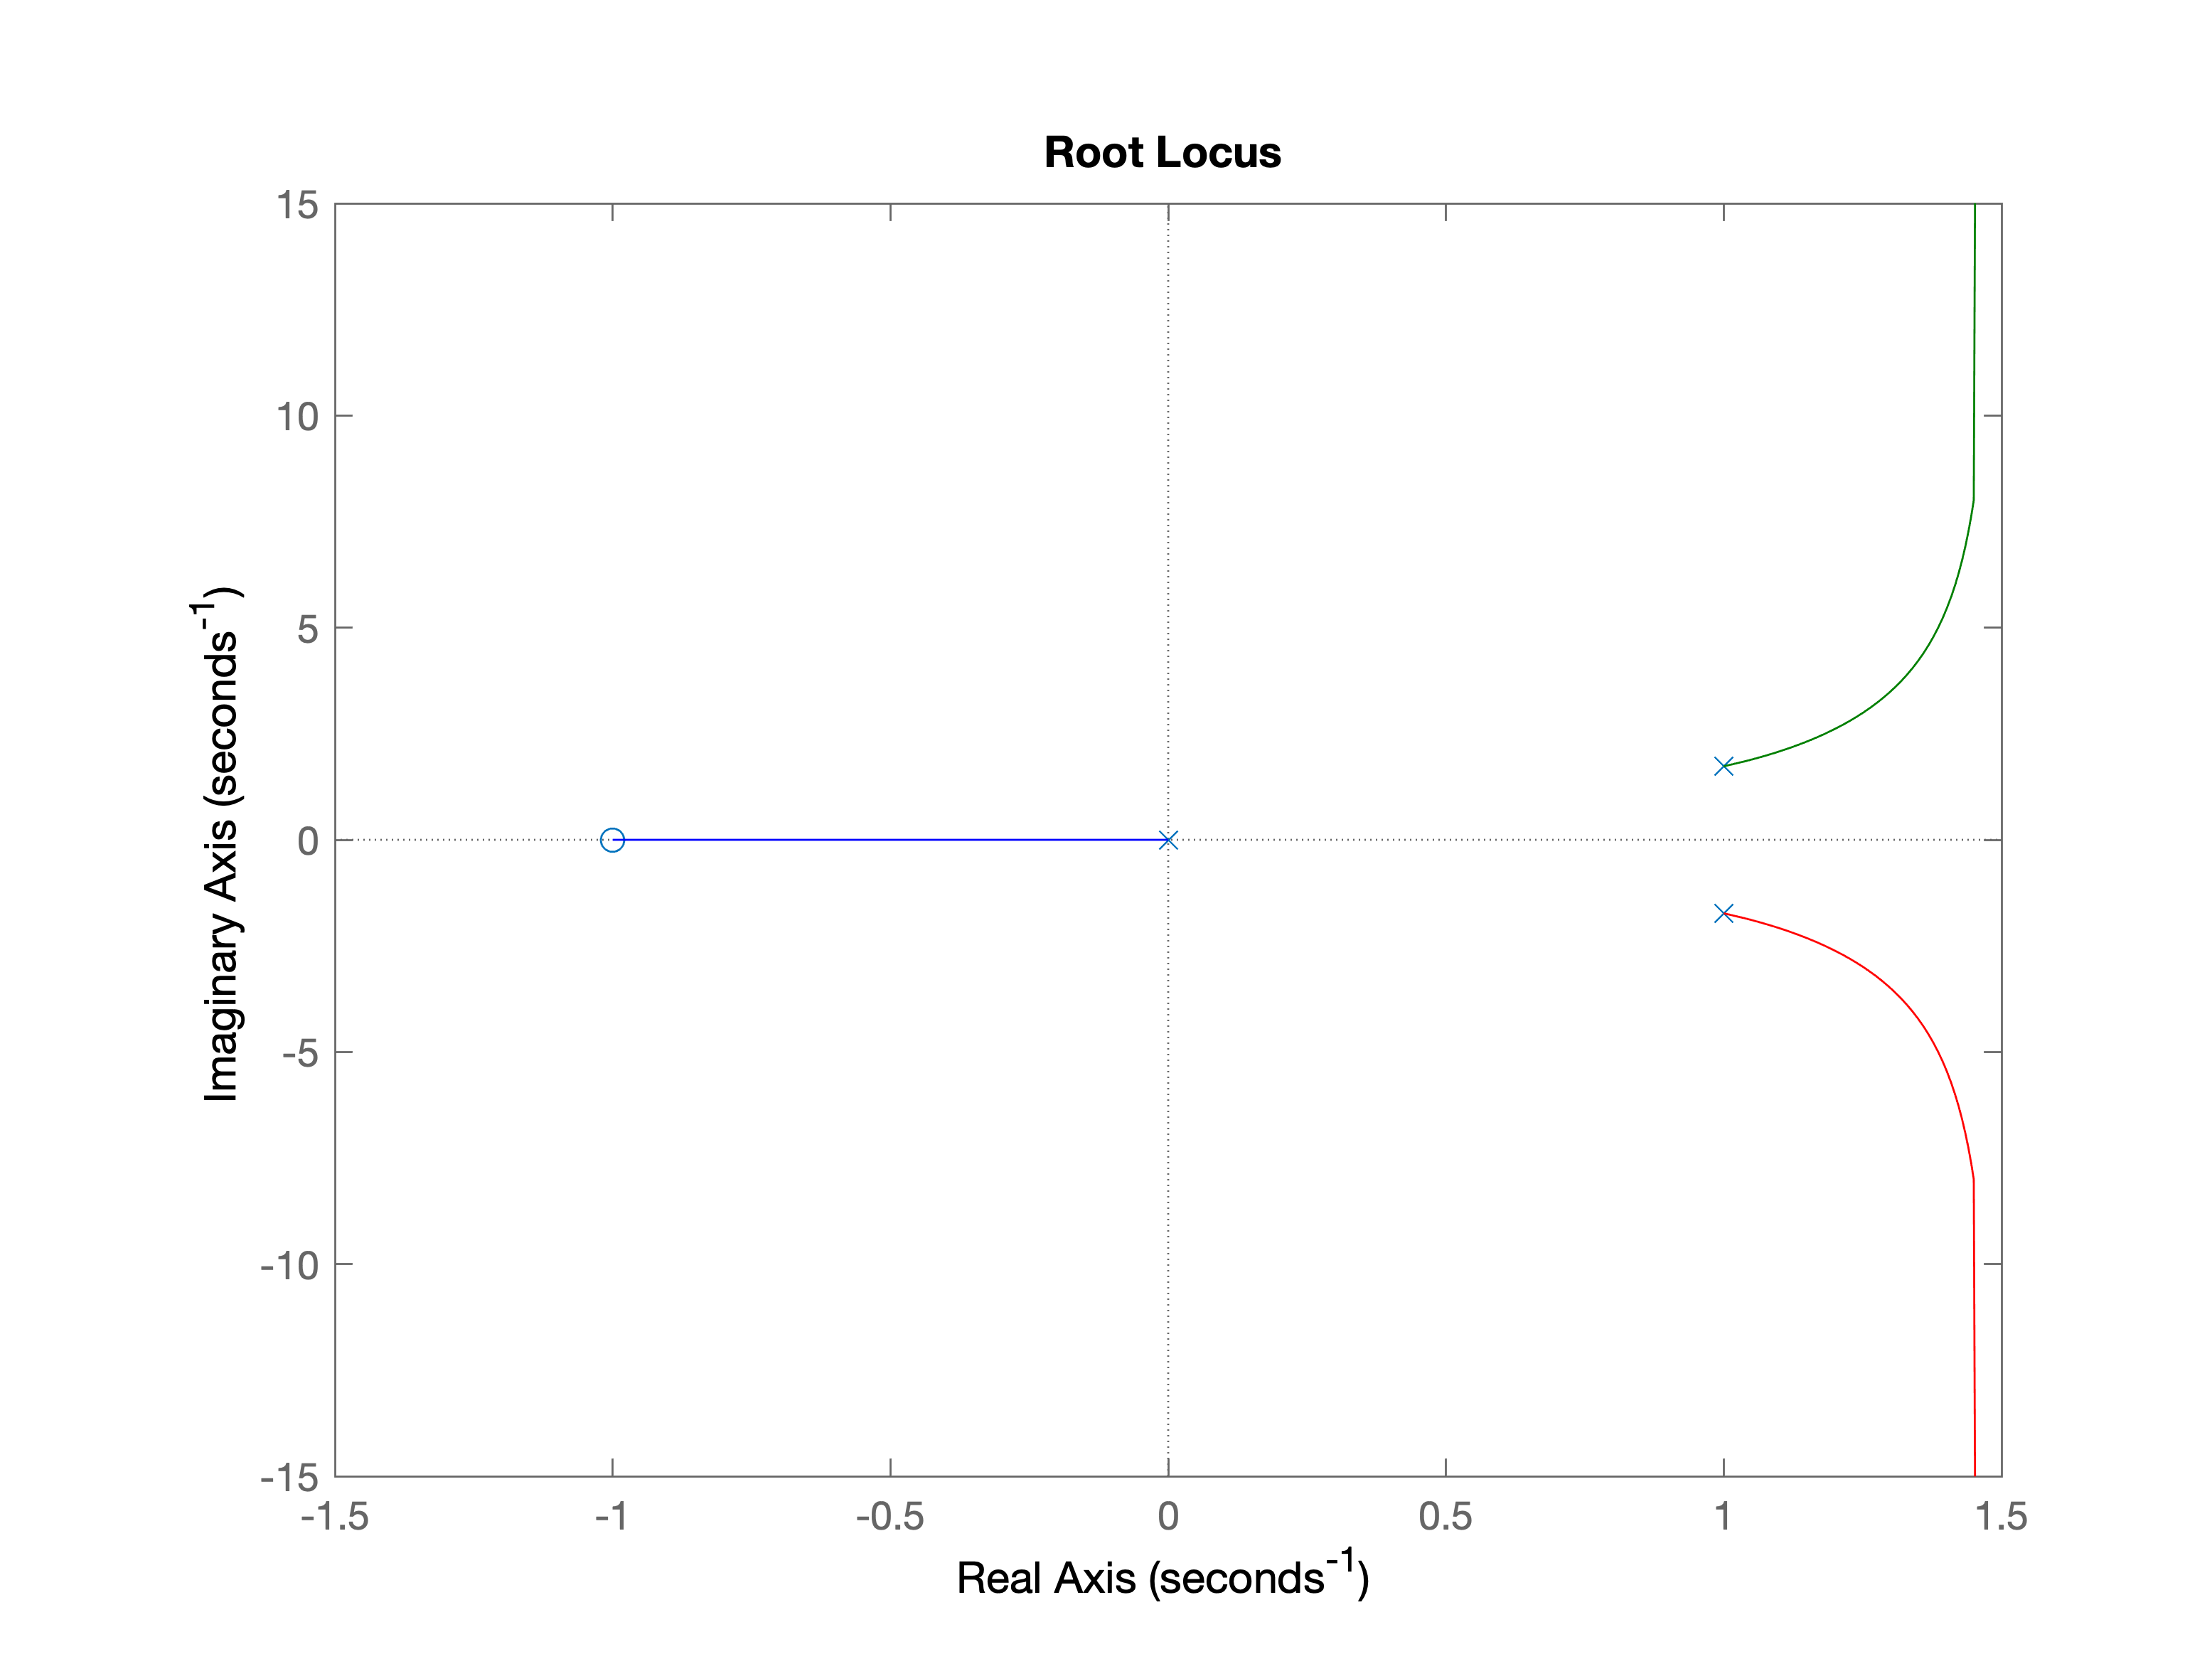
\includegraphics[width=12cm]{../Figure/Q1/Q1_b/I/rlocus.png}
	\end{figure}
	\item step response for closeloop system with I controller
	\begin{figure}[H]
		\caption{step response for closeloop system}
		\centering
		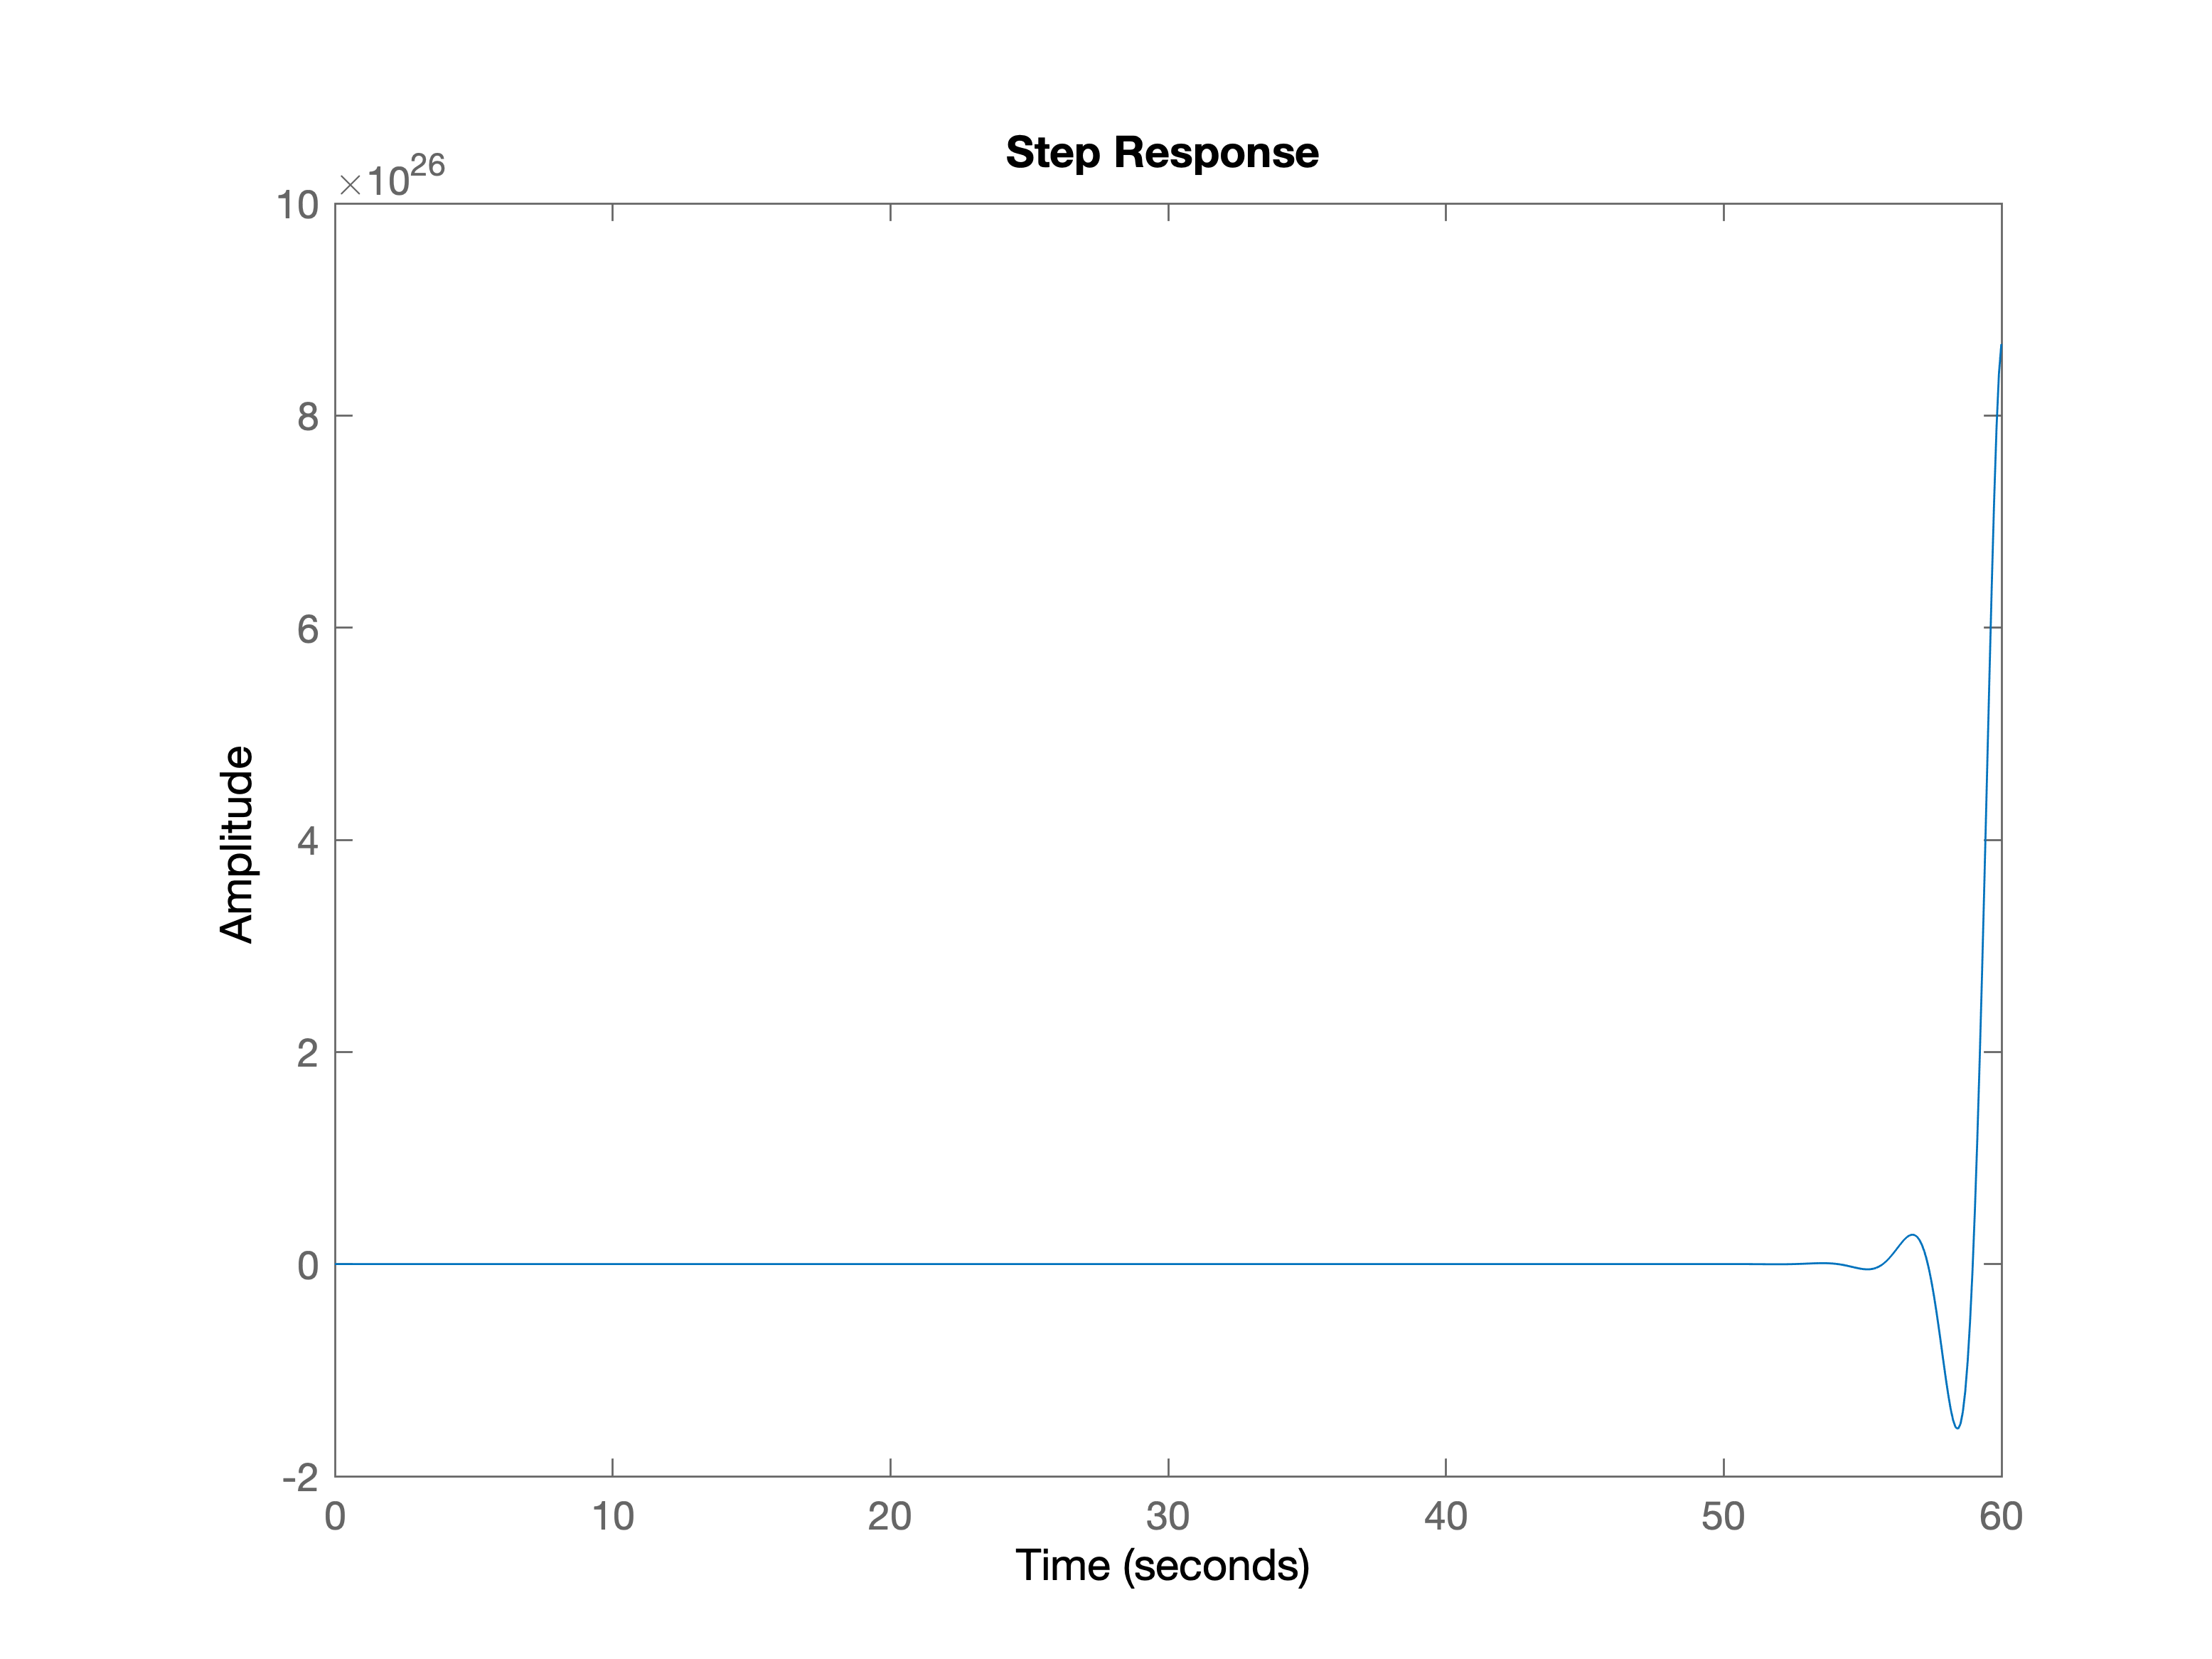
\includegraphics[width=12cm]{../Figure/Q1/Q1_b/I/feedback_step.png}
	\end{figure}
	\item closeloop bode (magnitude) with I controller
	\begin{figure}[H]
		\caption{closeloop bode (magnitude)}
		\centering
		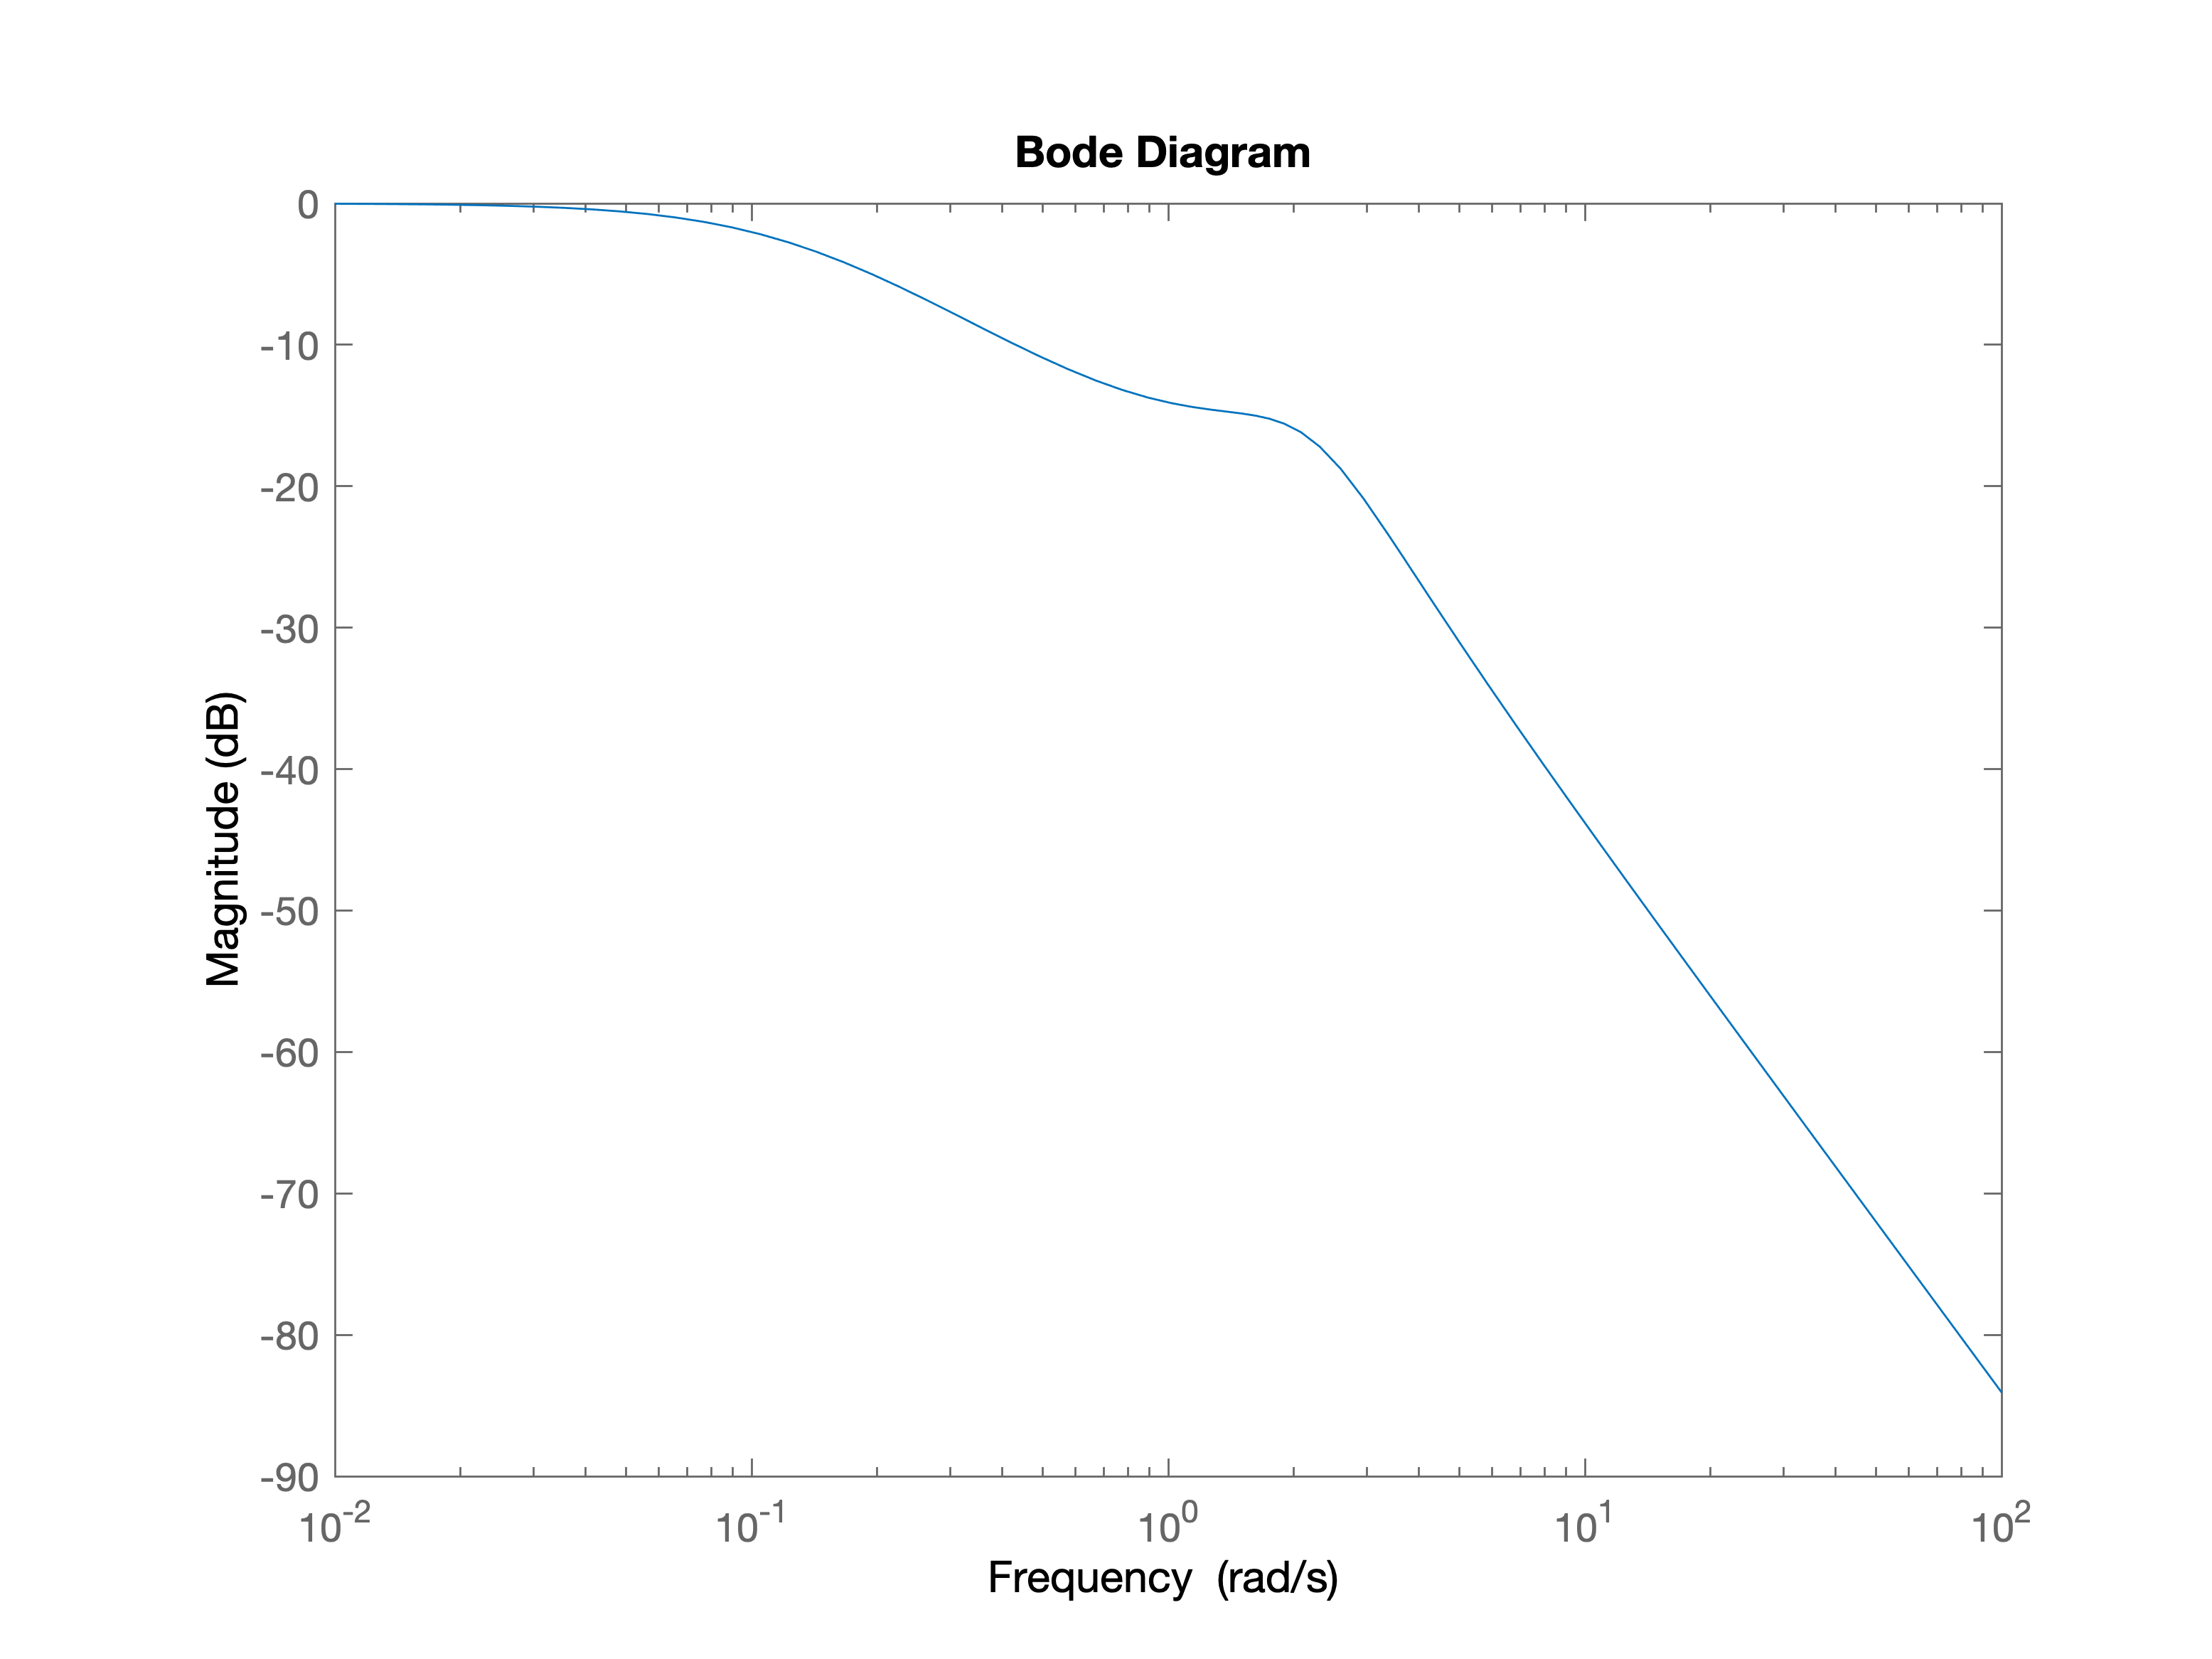
\includegraphics[width=12cm]{../Figure/Q1/Q1_b/I/feedback_bode.png}
	\end{figure}
	\item openloop bode (magnitude) with I controller
	\begin{figure}[H]
		\caption{openloop bode (magnitude)}
		\centering
		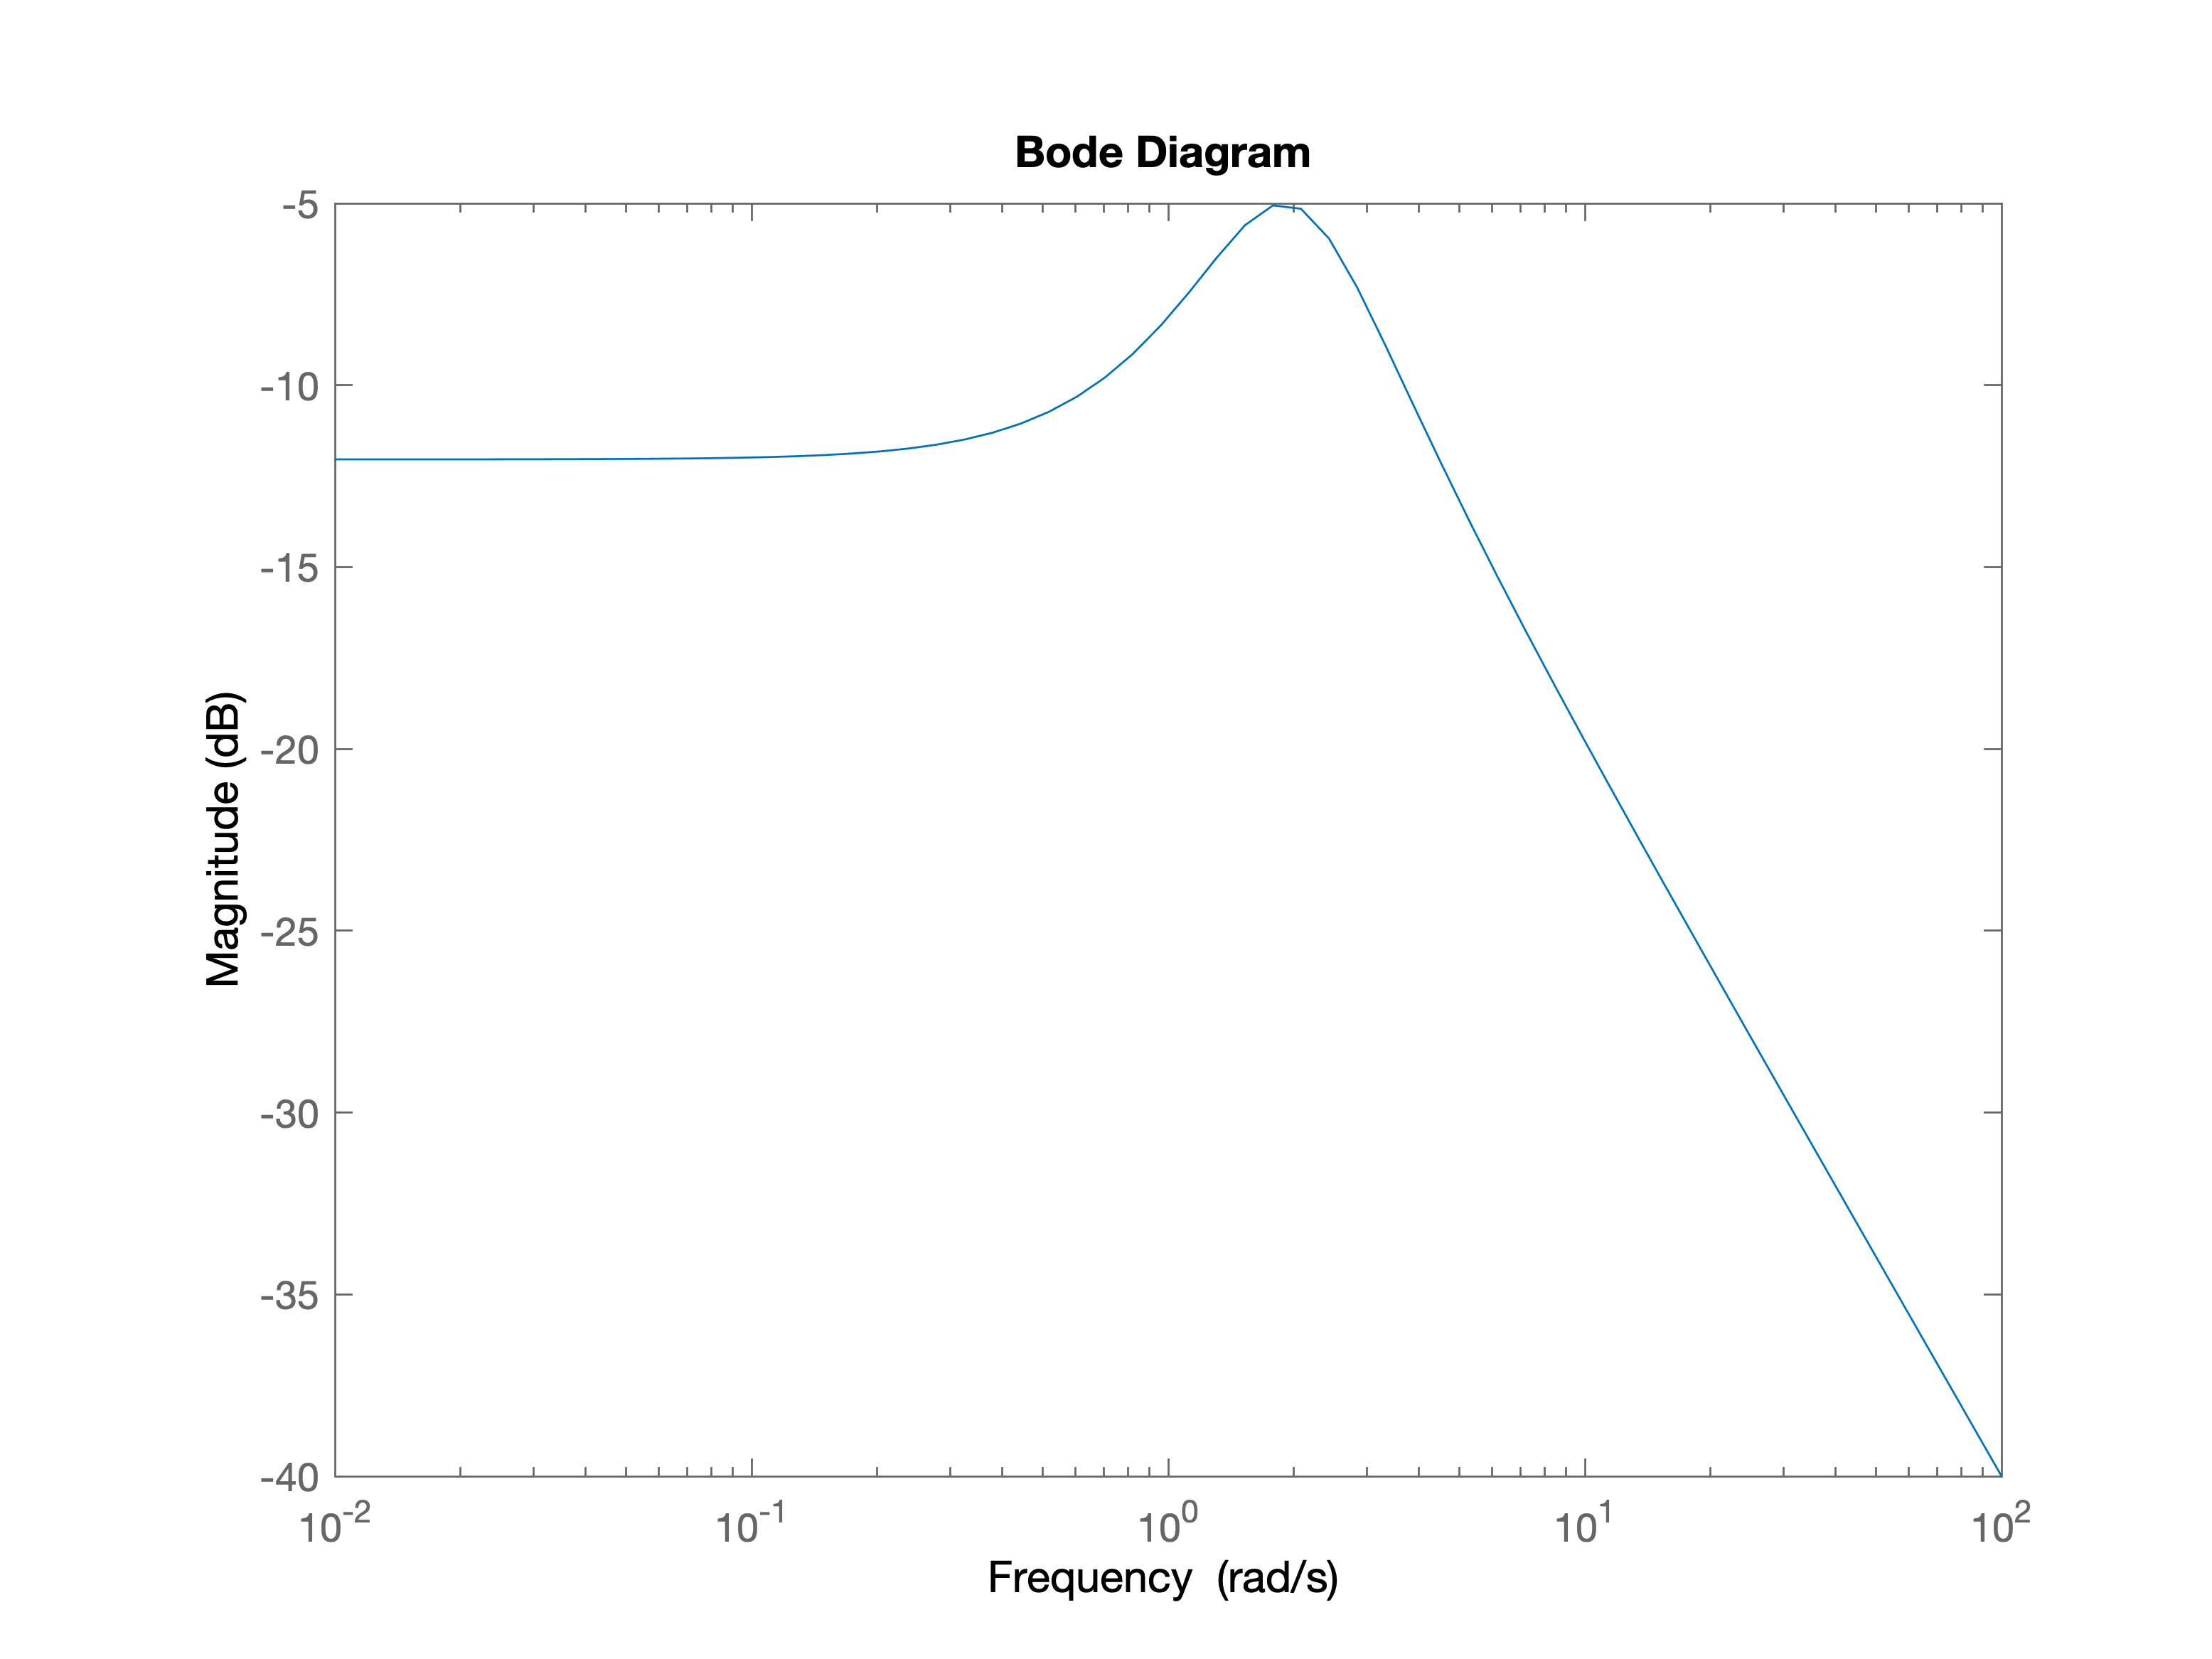
\includegraphics[width=12cm]{../Figure/Q1/Q1_b/I/openloop_bode.png}
	\end{figure}
	\item sensitivity function with I controller
	\begin{figure}[H]
		\caption{sensitivity function}
		\centering
		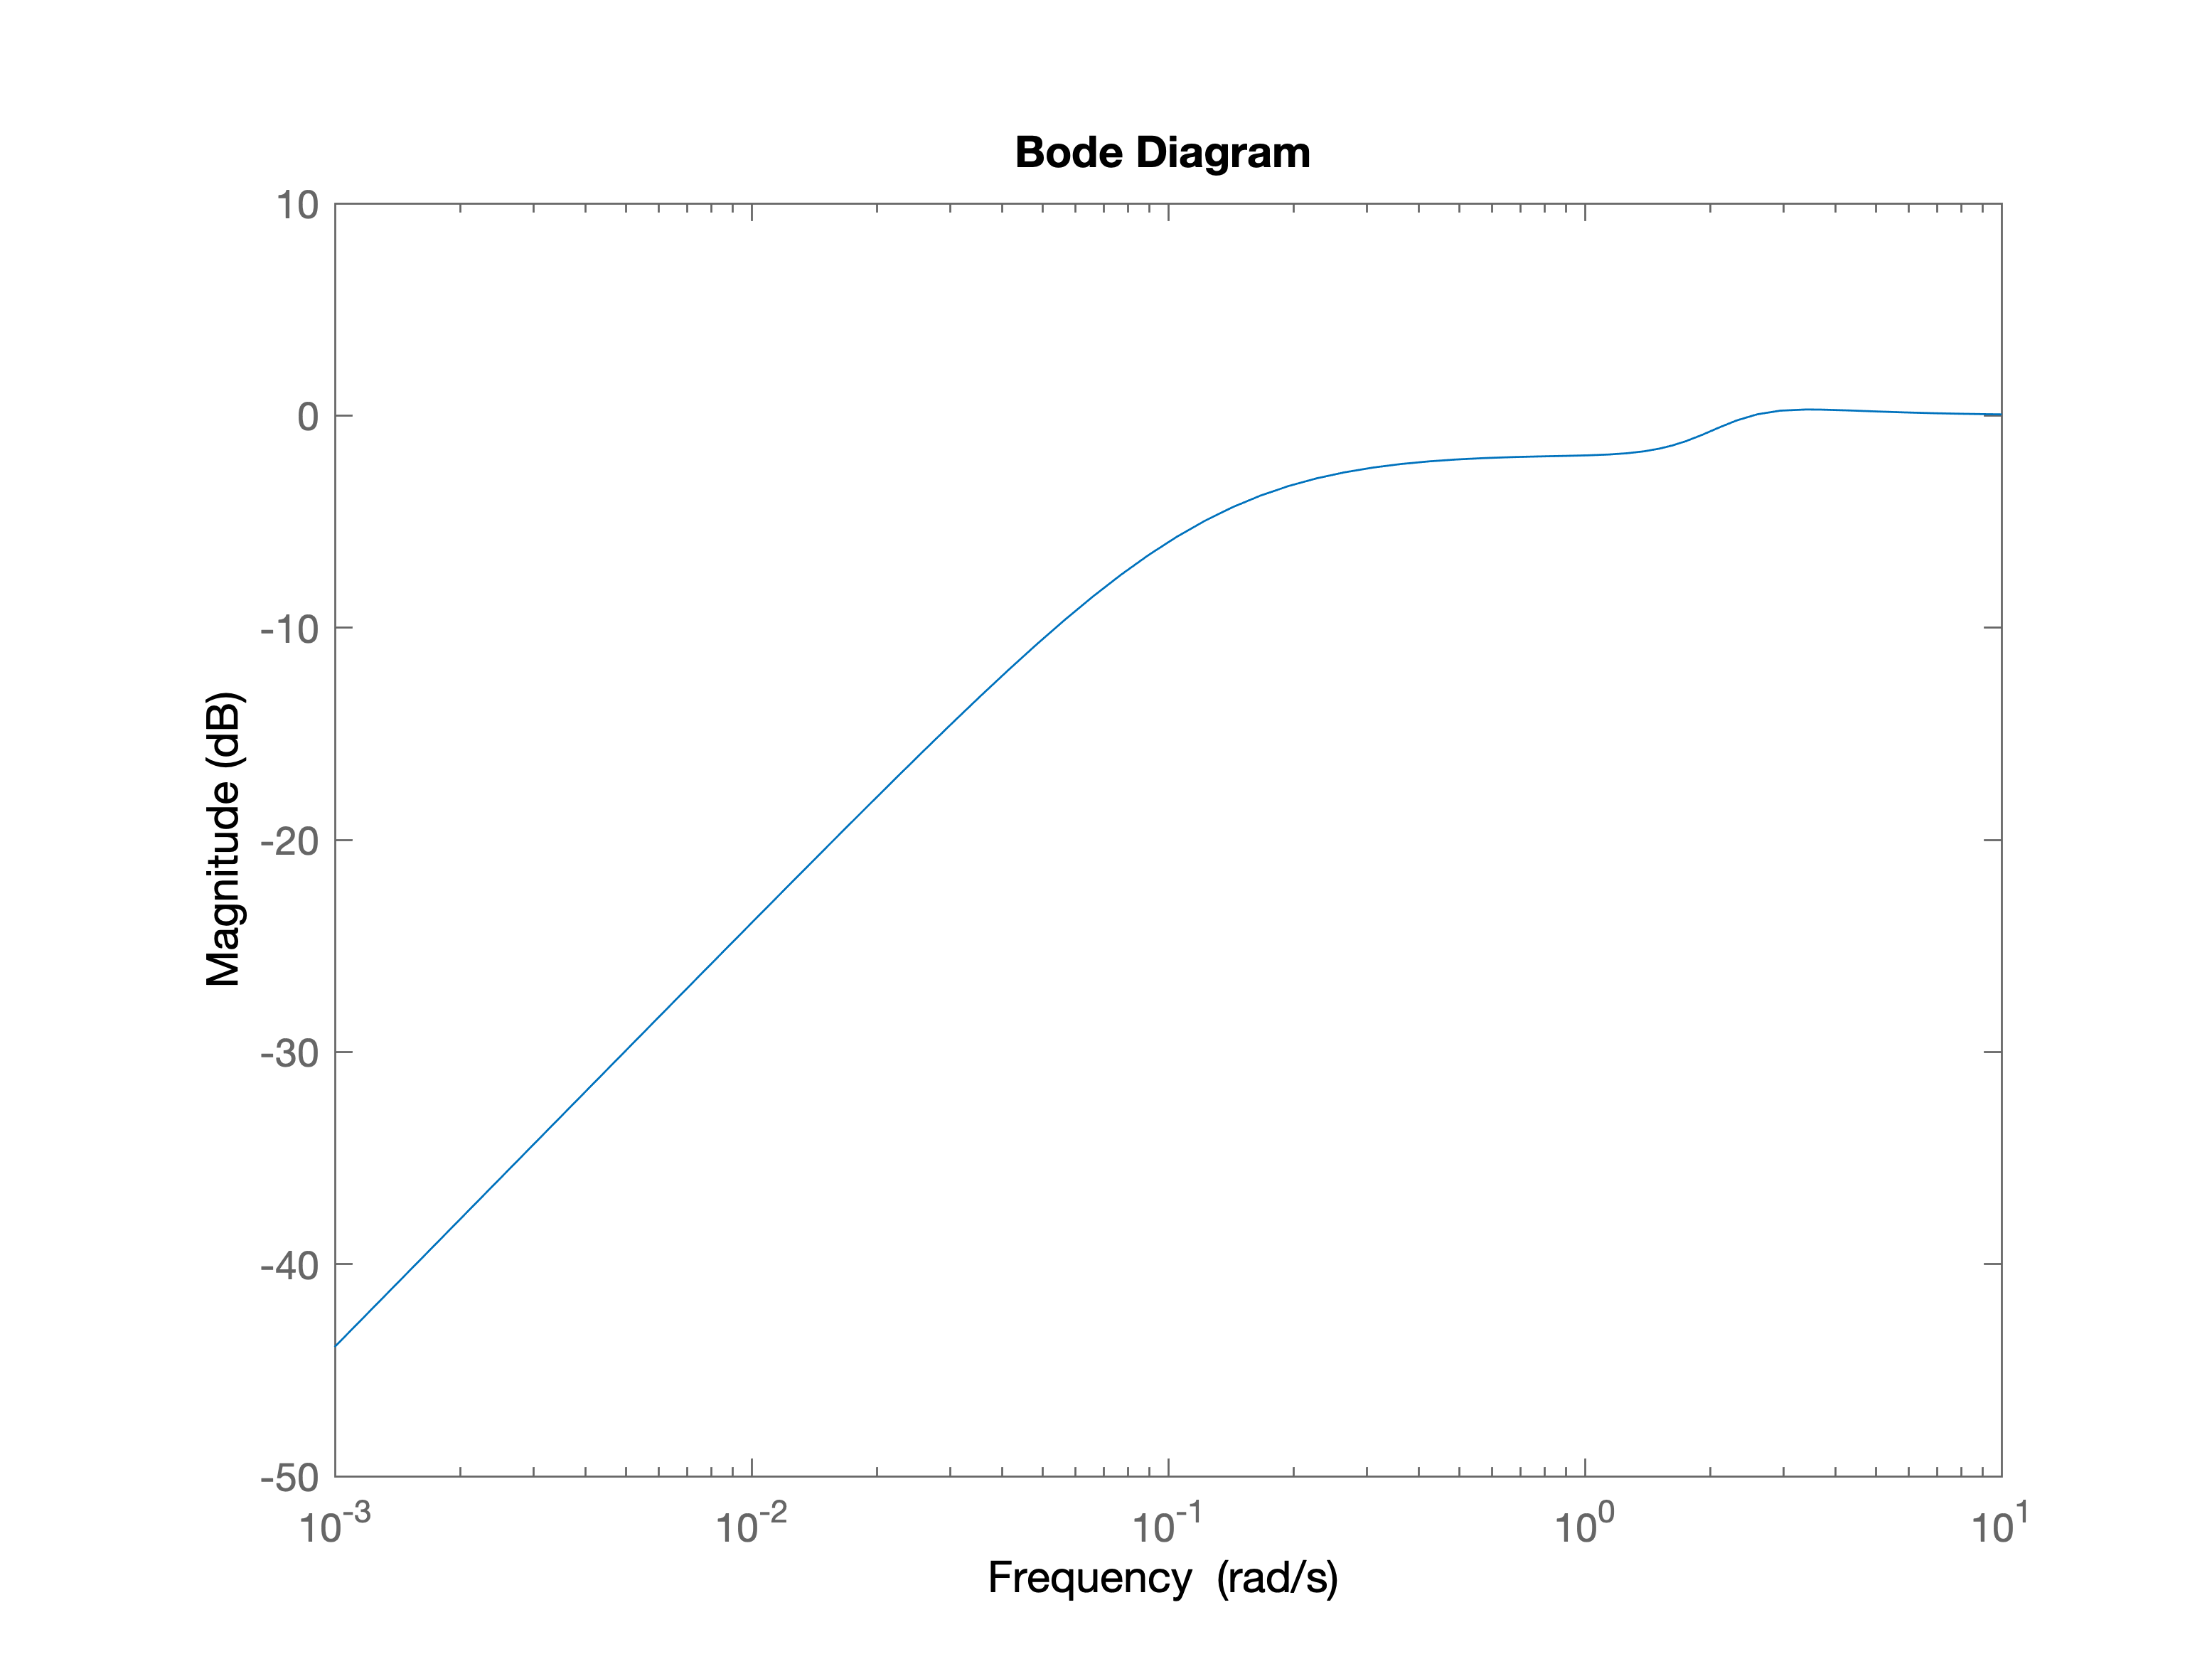
\includegraphics[width=12cm]{../Figure/Q1/Q1_b/I/s_bode.png}
	\end{figure}
	\item complementary sensitivity function with I controller
	\begin{figure}[H]
		\caption{complementary sensitivity function}
		\centering
		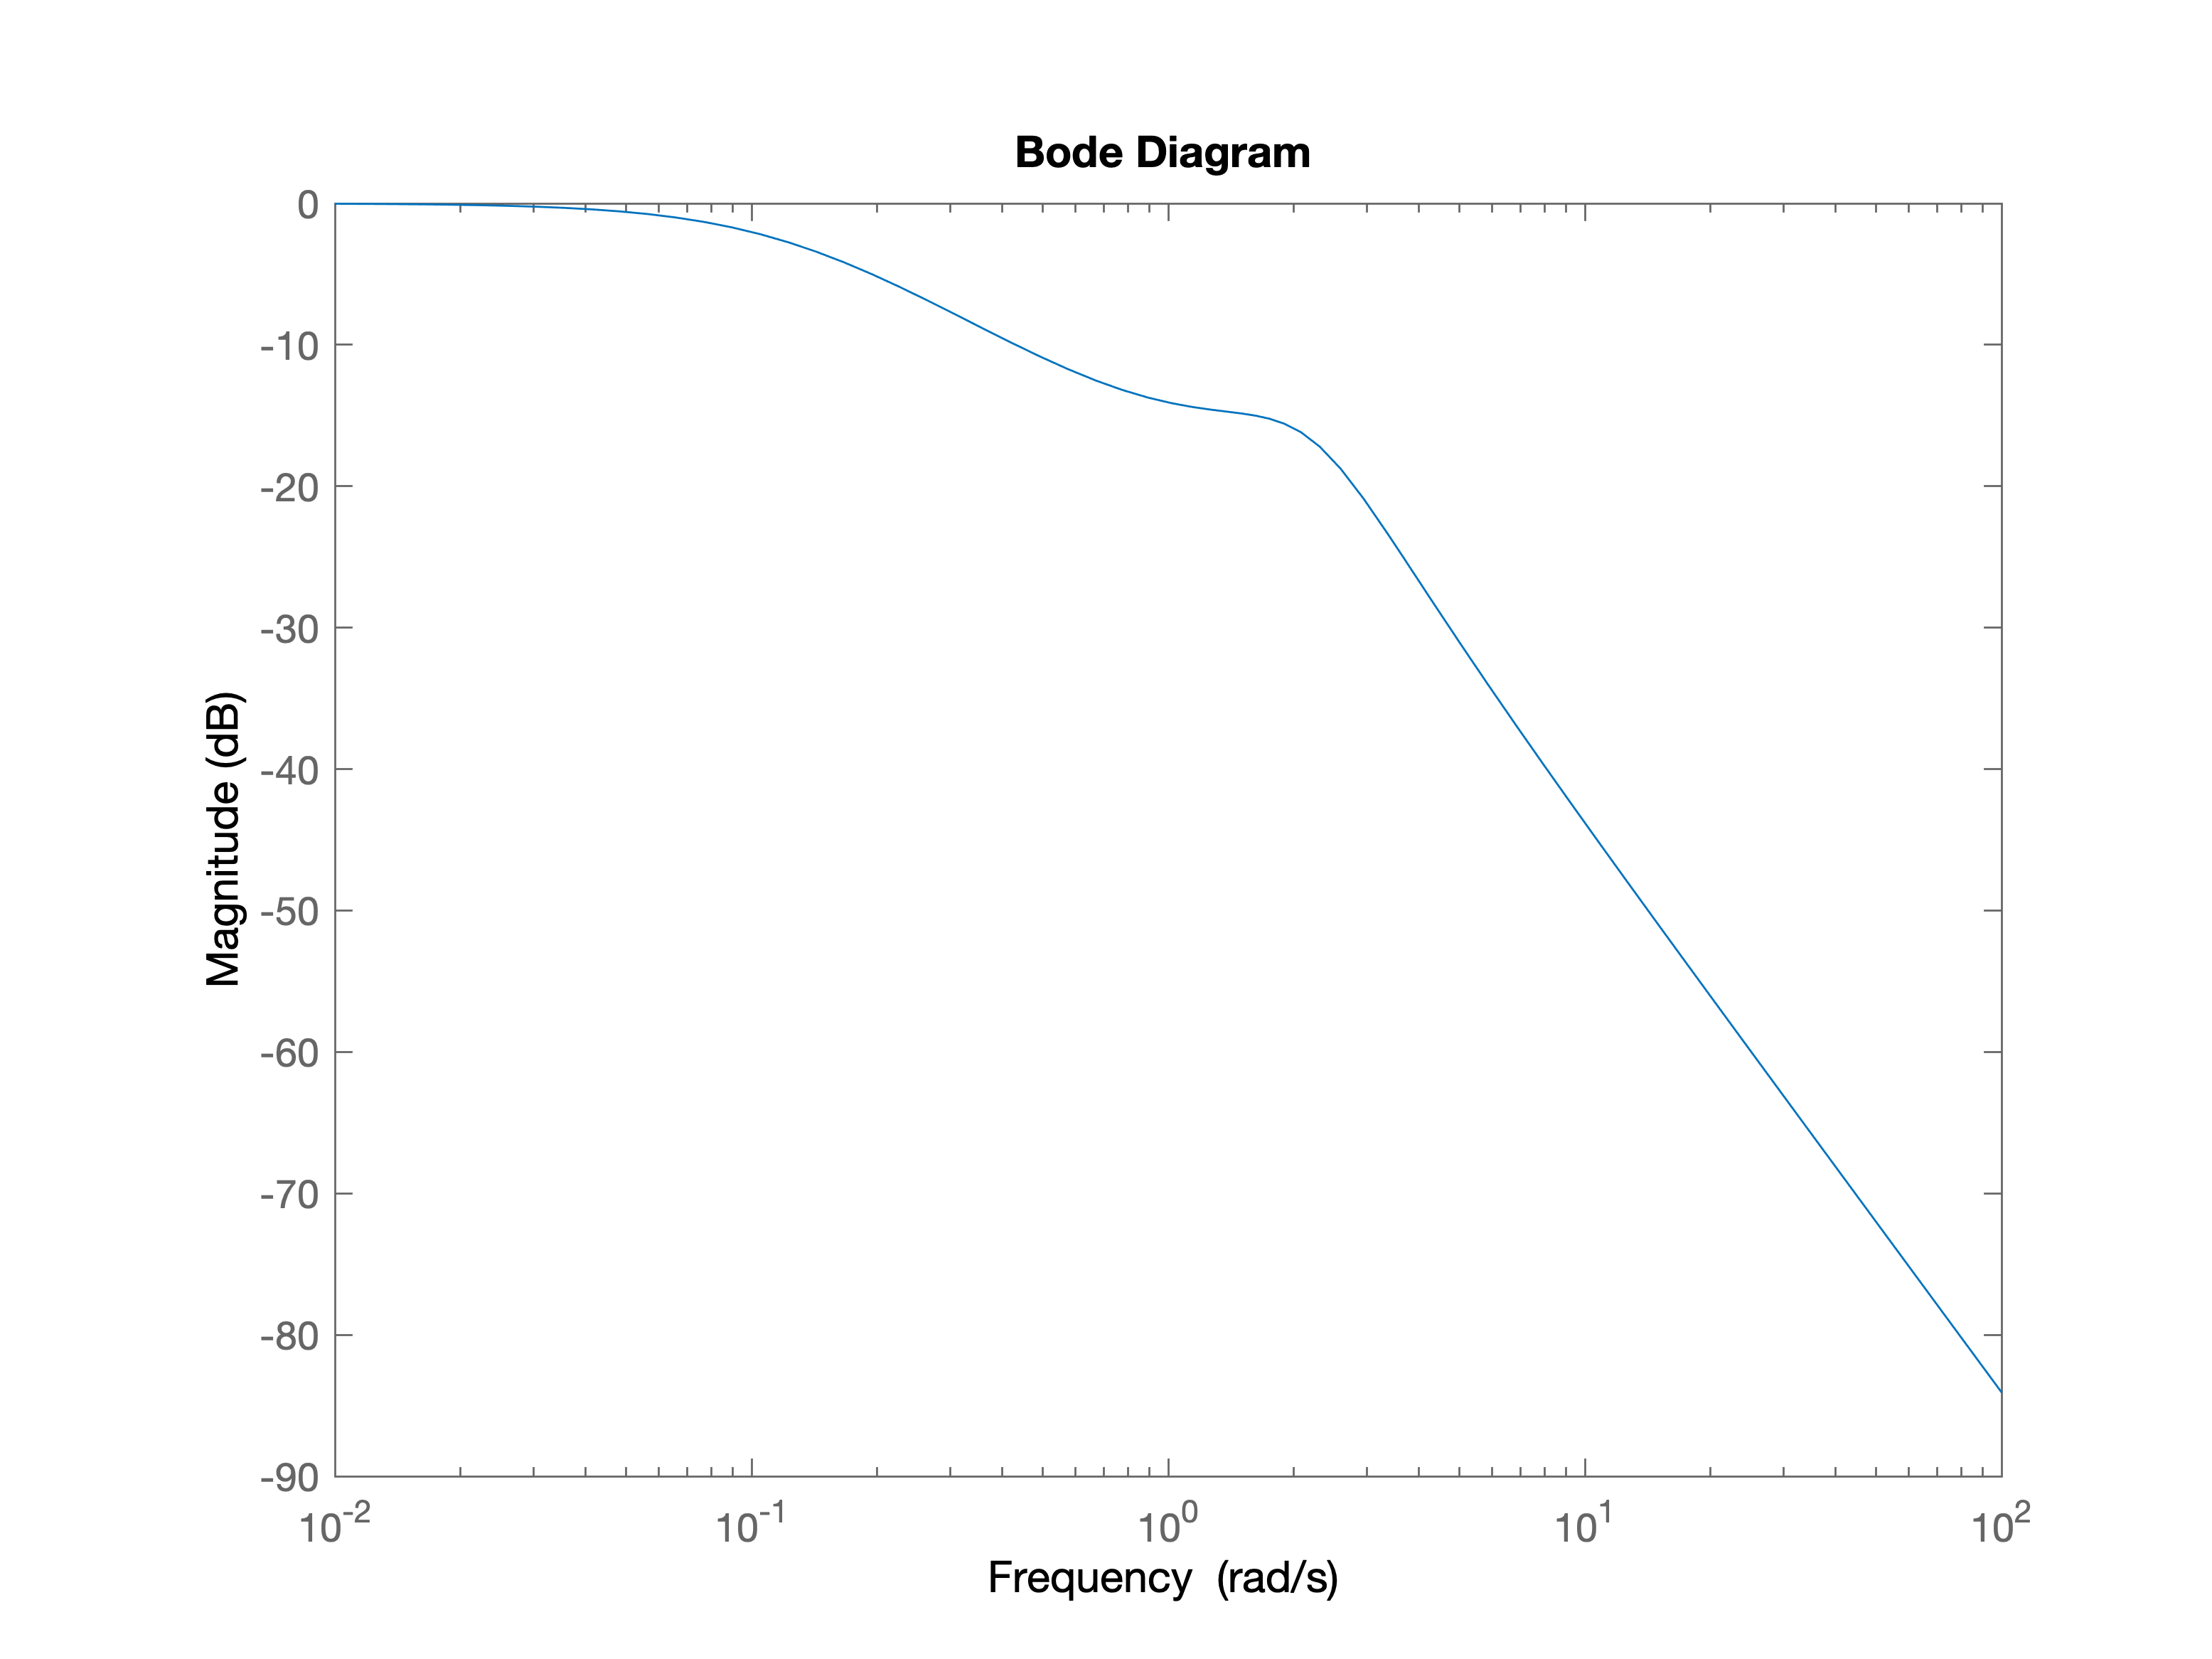
\includegraphics[width=12cm]{../Figure/Q1/Q1_b/I/t_bode.png}
	\end{figure}
\end{itemize}
system is always unstable.